\documentclass[twoside]{book}

% Packages required by doxygen
\usepackage{calc}
\usepackage{doxygen}
\usepackage{graphicx}
\usepackage[utf8]{inputenc}
\usepackage{makeidx}
\usepackage{multicol}
\usepackage{multirow}
\usepackage{fixltx2e}
\PassOptionsToPackage{warn}{textcomp}
\usepackage{textcomp}
\usepackage[nointegrals]{wasysym}
\usepackage[table]{xcolor}

% Font selection
\usepackage[T1]{fontenc}
\usepackage{mathptmx}
\usepackage[scaled=.90]{helvet}
\usepackage{courier}
\usepackage{amssymb}
\usepackage{sectsty}
\renewcommand{\familydefault}{\sfdefault}
\allsectionsfont{%
  \fontseries{bc}\selectfont%
  \color{darkgray}%
}
\renewcommand{\DoxyLabelFont}{%
  \fontseries{bc}\selectfont%
  \color{darkgray}%
}
\newcommand{\+}{\discretionary{\mbox{\scriptsize$\hookleftarrow$}}{}{}}

% Page & text layout
\usepackage{geometry}
\geometry{%
  a4paper,%
  top=2.5cm,%
  bottom=2.5cm,%
  left=2.5cm,%
  right=2.5cm%
}
\tolerance=750
\hfuzz=15pt
\hbadness=750
\setlength{\emergencystretch}{15pt}
\setlength{\parindent}{0cm}
\setlength{\parskip}{0.2cm}
\makeatletter
\renewcommand{\paragraph}{%
  \@startsection{paragraph}{4}{0ex}{-1.0ex}{1.0ex}{%
    \normalfont\normalsize\bfseries\SS@parafont%
  }%
}
\renewcommand{\subparagraph}{%
  \@startsection{subparagraph}{5}{0ex}{-1.0ex}{1.0ex}{%
    \normalfont\normalsize\bfseries\SS@subparafont%
  }%
}
\makeatother

% Headers & footers
\usepackage{fancyhdr}
\pagestyle{fancyplain}
\fancyhead[LE]{\fancyplain{}{\bfseries\thepage}}
\fancyhead[CE]{\fancyplain{}{}}
\fancyhead[RE]{\fancyplain{}{\bfseries\leftmark}}
\fancyhead[LO]{\fancyplain{}{\bfseries\rightmark}}
\fancyhead[CO]{\fancyplain{}{}}
\fancyhead[RO]{\fancyplain{}{\bfseries\thepage}}
\fancyfoot[LE]{\fancyplain{}{}}
\fancyfoot[CE]{\fancyplain{}{}}
\fancyfoot[RE]{\fancyplain{}{\bfseries\scriptsize Generated on Fri Jun 20 2014 11\+:38\+:38 for Include\+Dependencies\+Demo by Doxygen }}
\fancyfoot[LO]{\fancyplain{}{\bfseries\scriptsize Generated on Fri Jun 20 2014 11\+:38\+:38 for Include\+Dependencies\+Demo by Doxygen }}
\fancyfoot[CO]{\fancyplain{}{}}
\fancyfoot[RO]{\fancyplain{}{}}
\renewcommand{\footrulewidth}{0.4pt}
\renewcommand{\chaptermark}[1]{%
  \markboth{#1}{}%
}
\renewcommand{\sectionmark}[1]{%
  \markright{\thesection\ #1}%
}

% Indices & bibliography
\usepackage{natbib}
\usepackage[titles]{tocloft}
\setcounter{tocdepth}{3}
\setcounter{secnumdepth}{5}
\makeindex

% Hyperlinks (required, but should be loaded last)
\usepackage{ifpdf}
\ifpdf
  \usepackage[pdftex,pagebackref=true]{hyperref}
\else
  \usepackage[ps2pdf,pagebackref=true]{hyperref}
\fi
\hypersetup{%
  colorlinks=true,%
  linkcolor=blue,%
  citecolor=blue,%
  unicode%
}

% Custom commands
\newcommand{\clearemptydoublepage}{%
  \newpage{\pagestyle{empty}\cleardoublepage}%
}


%===== C O N T E N T S =====

\begin{document}

% Titlepage & ToC
\hypersetup{pageanchor=false,
             bookmarks=true,
             bookmarksnumbered=true,
             pdfencoding=unicode
            }
\pagenumbering{roman}
\begin{titlepage}
\vspace*{7cm}
\begin{center}%
{\Large Include\+Dependencies\+Demo }\\
\vspace*{1cm}
{\large Generated by Doxygen 1.8.7}\\
\vspace*{0.5cm}
{\small Fri Jun 20 2014 11:38:38}\\
\end{center}
\end{titlepage}
\clearemptydoublepage
\tableofcontents
\clearemptydoublepage
\pagenumbering{arabic}
\hypersetup{pageanchor=true}

%--- Begin generated contents ---
\chapter{include\+Dependencies\+Demo}
\label{md__home_gernot_src_github_include_dependencies_demo__r_e_a_d_m_e}
\hypertarget{md__home_gernot_src_github_include_dependencies_demo__r_e_a_d_m_e}{}
\input{md__home_gernot_src_github_include_dependencies_demo__r_e_a_d_m_e}
\chapter{File Index}
\section{File List}
Here is a list of all files with brief descriptions\+:\begin{DoxyCompactList}
\item\contentsline{section}{/home/gernot/src/github/include\+Dependencies\+Demo/\hyperlink{a_8h}{a.\+h} }{\pageref{a_8h}}{}
\item\contentsline{section}{/home/gernot/src/github/include\+Dependencies\+Demo/\hyperlink{b_8h}{b.\+h} }{\pageref{b_8h}}{}
\item\contentsline{section}{/home/gernot/src/github/include\+Dependencies\+Demo/\hyperlink{c_8h}{c.\+h} }{\pageref{c_8h}}{}
\item\contentsline{section}{/home/gernot/src/github/include\+Dependencies\+Demo/\hyperlink{d_8h}{d.\+h} }{\pageref{d_8h}}{}
\item\contentsline{section}{/home/gernot/src/github/include\+Dependencies\+Demo/\hyperlink{main_8cpp}{main.\+cpp} }{\pageref{main_8cpp}}{}
\end{DoxyCompactList}

\chapter{File Documentation}
\hypertarget{a_8h}{\section{/home/gernot/src/github/include\+Dependencies\+Demo/a.h File Reference}
\label{a_8h}\index{/home/gernot/src/github/include\+Dependencies\+Demo/a.\+h@{/home/gernot/src/github/include\+Dependencies\+Demo/a.\+h}}
}
{\ttfamily \#include \char`\"{}b.\+h\char`\"{}}\\*
Include dependency graph for a.\+h\+:\nopagebreak
\begin{figure}[H]
\begin{center}
\leavevmode
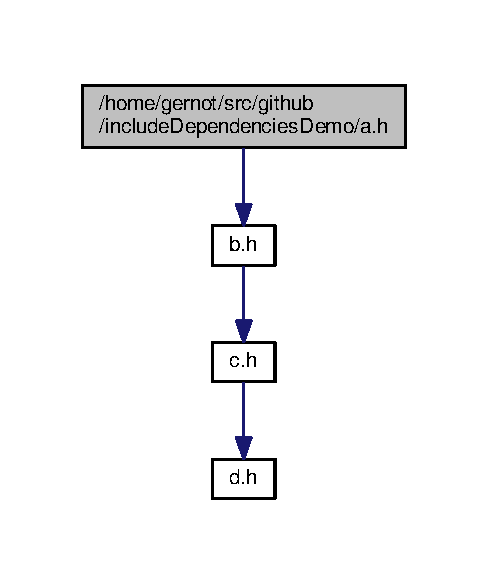
\includegraphics[width=234pt]{a_8h__incl}
\end{center}
\end{figure}
This graph shows which files directly or indirectly include this file\+:\nopagebreak
\begin{figure}[H]
\begin{center}
\leavevmode
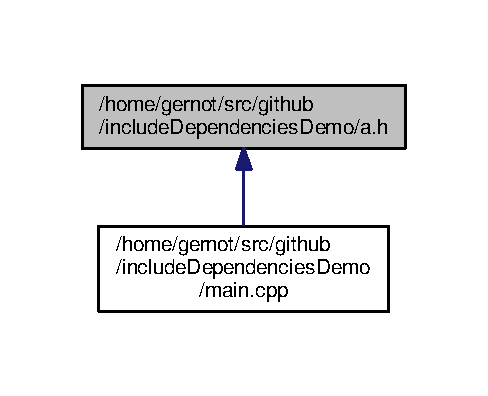
\includegraphics[width=234pt]{a_8h__dep__incl}
\end{center}
\end{figure}
\subsection*{Functions}
\begin{DoxyCompactItemize}
\item 
void \hyperlink{a_8h_a3b750b68a7a31daf9f67711bd47d0a18}{func\+A} ()
\end{DoxyCompactItemize}


\subsection{Function Documentation}
\hypertarget{a_8h_a3b750b68a7a31daf9f67711bd47d0a18}{\index{a.\+h@{a.\+h}!func\+A@{func\+A}}
\index{func\+A@{func\+A}!a.\+h@{a.\+h}}
\subsubsection[{func\+A}]{\setlength{\rightskip}{0pt plus 5cm}void func\+A (
\begin{DoxyParamCaption}
{}
\end{DoxyParamCaption}
)}}\label{a_8h_a3b750b68a7a31daf9f67711bd47d0a18}

\hypertarget{b_8h}{\section{/home/gernot/src/github/include\+Dependencies\+Demo/b.h File Reference}
\label{b_8h}\index{/home/gernot/src/github/include\+Dependencies\+Demo/b.\+h@{/home/gernot/src/github/include\+Dependencies\+Demo/b.\+h}}
}
{\ttfamily \#include \char`\"{}c.\+h\char`\"{}}\\*
Include dependency graph for b.\+h\+:\nopagebreak
\begin{figure}[H]
\begin{center}
\leavevmode
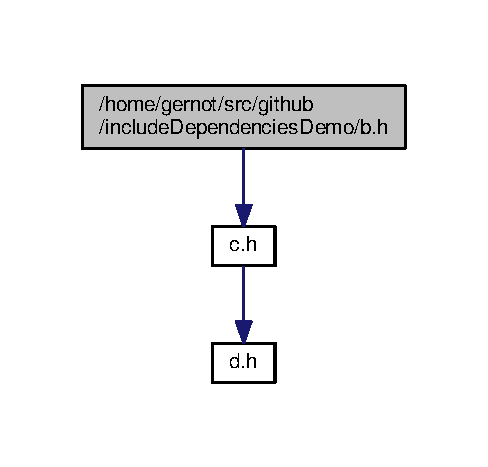
\includegraphics[width=234pt]{b_8h__incl}
\end{center}
\end{figure}
This graph shows which files directly or indirectly include this file\+:\nopagebreak
\begin{figure}[H]
\begin{center}
\leavevmode
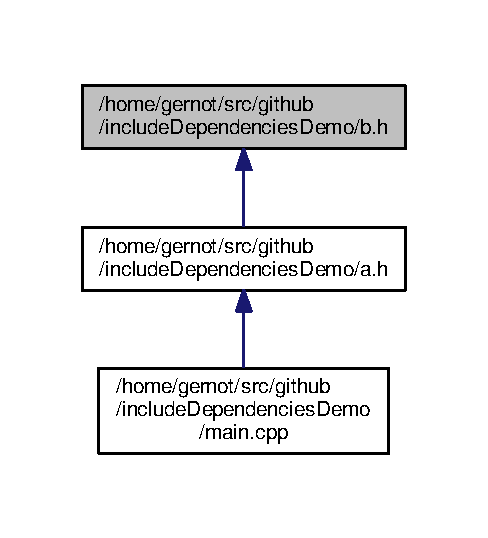
\includegraphics[width=234pt]{b_8h__dep__incl}
\end{center}
\end{figure}
\subsection*{Functions}
\begin{DoxyCompactItemize}
\item 
int \hyperlink{b_8h_acf62575dc784a101049c381bb636b1d1}{func\+B} ()
\end{DoxyCompactItemize}


\subsection{Function Documentation}
\hypertarget{b_8h_acf62575dc784a101049c381bb636b1d1}{\index{b.\+h@{b.\+h}!func\+B@{func\+B}}
\index{func\+B@{func\+B}!b.\+h@{b.\+h}}
\subsubsection[{func\+B}]{\setlength{\rightskip}{0pt plus 5cm}int func\+B (
\begin{DoxyParamCaption}
{}
\end{DoxyParamCaption}
)}}\label{b_8h_acf62575dc784a101049c381bb636b1d1}

\hypertarget{c_8h}{\section{/home/gernot/src/github/include\+Dependencies\+Demo/c.h File Reference}
\label{c_8h}\index{/home/gernot/src/github/include\+Dependencies\+Demo/c.\+h@{/home/gernot/src/github/include\+Dependencies\+Demo/c.\+h}}
}
{\ttfamily \#include \char`\"{}d.\+h\char`\"{}}\\*
Include dependency graph for c.\+h\+:\nopagebreak
\begin{figure}[H]
\begin{center}
\leavevmode
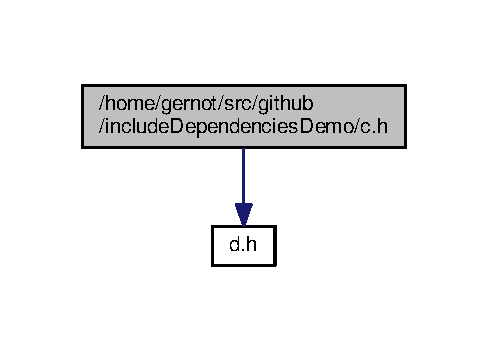
\includegraphics[width=234pt]{c_8h__incl}
\end{center}
\end{figure}
This graph shows which files directly or indirectly include this file\+:\nopagebreak
\begin{figure}[H]
\begin{center}
\leavevmode
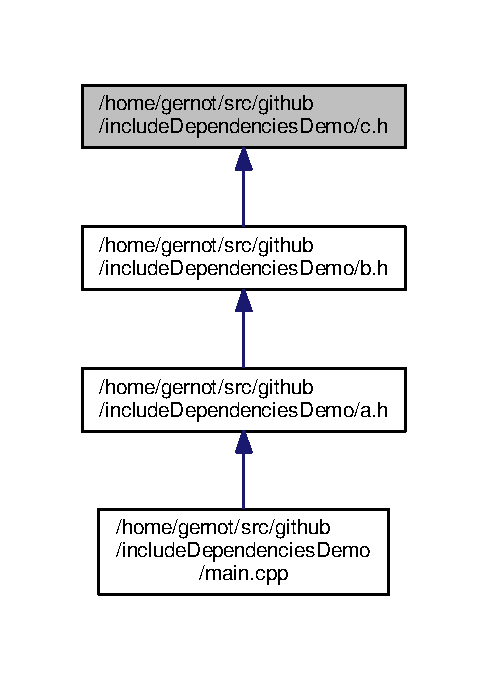
\includegraphics[width=234pt]{c_8h__dep__incl}
\end{center}
\end{figure}
\subsection*{Functions}
\begin{DoxyCompactItemize}
\item 
void \hyperlink{c_8h_a44a9ecb5c045e7dcb6f50dac669dab87}{func\+C} ()
\end{DoxyCompactItemize}


\subsection{Function Documentation}
\hypertarget{c_8h_a44a9ecb5c045e7dcb6f50dac669dab87}{\index{c.\+h@{c.\+h}!func\+C@{func\+C}}
\index{func\+C@{func\+C}!c.\+h@{c.\+h}}
\subsubsection[{func\+C}]{\setlength{\rightskip}{0pt plus 5cm}void func\+C (
\begin{DoxyParamCaption}
{}
\end{DoxyParamCaption}
)}}\label{c_8h_a44a9ecb5c045e7dcb6f50dac669dab87}

\hypertarget{d_8h}{\section{/home/gernot/src/github/include\+Dependencies\+Demo/d.h File Reference}
\label{d_8h}\index{/home/gernot/src/github/include\+Dependencies\+Demo/d.\+h@{/home/gernot/src/github/include\+Dependencies\+Demo/d.\+h}}
}
This graph shows which files directly or indirectly include this file\+:\nopagebreak
\begin{figure}[H]
\begin{center}
\leavevmode
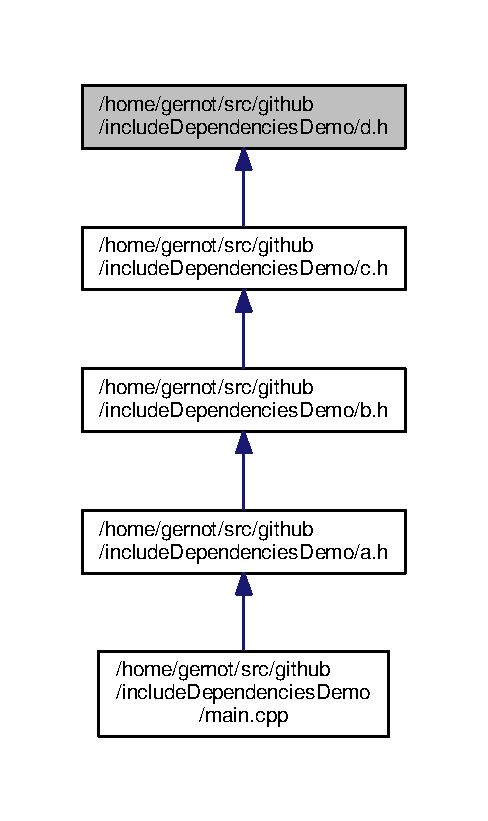
\includegraphics[width=234pt]{d_8h__dep__incl}
\end{center}
\end{figure}
\subsection*{Functions}
\begin{DoxyCompactItemize}
\item 
void \hyperlink{d_8h_a5144fe500d965ce32aab1915ad58dd2d}{func\+D1} ()
\item 
void \hyperlink{d_8h_a69aeb3c0b7146a247ba908a29c42830e}{func\+D2} ()
\end{DoxyCompactItemize}


\subsection{Function Documentation}
\hypertarget{d_8h_a5144fe500d965ce32aab1915ad58dd2d}{\index{d.\+h@{d.\+h}!func\+D1@{func\+D1}}
\index{func\+D1@{func\+D1}!d.\+h@{d.\+h}}
\subsubsection[{func\+D1}]{\setlength{\rightskip}{0pt plus 5cm}void func\+D1 (
\begin{DoxyParamCaption}
{}
\end{DoxyParamCaption}
)}}\label{d_8h_a5144fe500d965ce32aab1915ad58dd2d}
\hypertarget{d_8h_a69aeb3c0b7146a247ba908a29c42830e}{\index{d.\+h@{d.\+h}!func\+D2@{func\+D2}}
\index{func\+D2@{func\+D2}!d.\+h@{d.\+h}}
\subsubsection[{func\+D2}]{\setlength{\rightskip}{0pt plus 5cm}void func\+D2 (
\begin{DoxyParamCaption}
{}
\end{DoxyParamCaption}
)}}\label{d_8h_a69aeb3c0b7146a247ba908a29c42830e}

\hypertarget{main_8cpp}{\section{/home/gernot/src/github/include\+Dependencies\+Demo/main.cpp File Reference}
\label{main_8cpp}\index{/home/gernot/src/github/include\+Dependencies\+Demo/main.\+cpp@{/home/gernot/src/github/include\+Dependencies\+Demo/main.\+cpp}}
}
{\ttfamily \#include \char`\"{}a.\+h\char`\"{}}\\*
{\ttfamily \#include $<$iostream$>$}\\*
Include dependency graph for main.\+cpp\+:\nopagebreak
\begin{figure}[H]
\begin{center}
\leavevmode
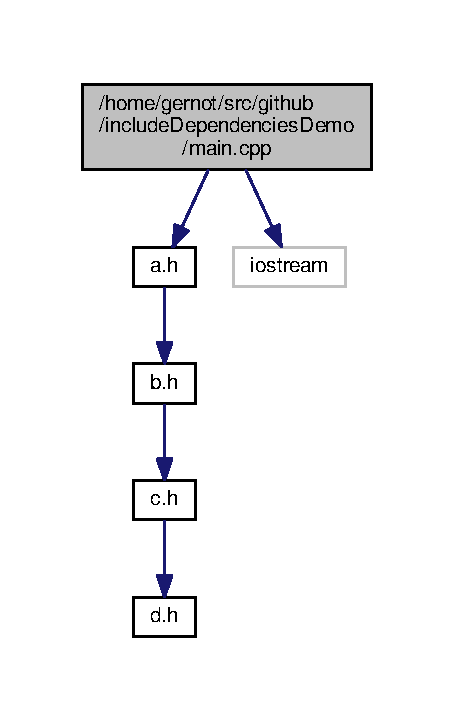
\includegraphics[width=218pt]{main_8cpp__incl}
\end{center}
\end{figure}
\subsection*{Functions}
\begin{DoxyCompactItemize}
\item 
int \hyperlink{main_8cpp_ae66f6b31b5ad750f1fe042a706a4e3d4}{main} ()
\end{DoxyCompactItemize}


\subsection{Function Documentation}
\hypertarget{main_8cpp_ae66f6b31b5ad750f1fe042a706a4e3d4}{\index{main.\+cpp@{main.\+cpp}!main@{main}}
\index{main@{main}!main.\+cpp@{main.\+cpp}}
\subsubsection[{main}]{\setlength{\rightskip}{0pt plus 5cm}int main (
\begin{DoxyParamCaption}
{}
\end{DoxyParamCaption}
)}}\label{main_8cpp_ae66f6b31b5ad750f1fe042a706a4e3d4}

\hypertarget{_r_e_a_d_m_e_8md}{\section{/home/gernot/src/github/include\+Dependencies\+Demo/\+R\+E\+A\+D\+M\+E.md File Reference}
\label{_r_e_a_d_m_e_8md}\index{/home/gernot/src/github/include\+Dependencies\+Demo/\+R\+E\+A\+D\+M\+E.\+md@{/home/gernot/src/github/include\+Dependencies\+Demo/\+R\+E\+A\+D\+M\+E.\+md}}
}

%--- End generated contents ---

% Index
\newpage
\phantomsection
\addcontentsline{toc}{chapter}{Index}
\printindex

\end{document}
